\chapter{Introducción y objetivos}\label{cap.introduccion}
El objetivo fundamental de este trabajo se sitúa en tratar de entender el funcionamiento del aprendizaje profundo con redes neuronales, utilizando para ello una de las diferentes plataformas existentes para el desarrollo de las mismas, Caffe.\\

En este capítulo se situará el trabajo en el marco existente en la actualidad, explicando de manera genérica en qué consiste el aprendizaje profundo, el por qué del uso de una determinada plataforma y los problemas que es posible abordar con esta técnica. Además, se expondrán los objetivos de este proyecto, la metodología empleada para alcanzarlos y un pequeño resumen de cómo se ha estructurado el trabajo.

\section{Contexto y motivación}

Desde que los primeros ordenadores fueron programados, el ser humano se ha planteado la posibilidad de conseguir que estas máquinas adquieran inteligencia, logrando que realicen tareas propias de las personas permitiendo, por ejemplo, automatizar el trabajo de rutina, entender el habla o las imágenes, hacer diagnósticos en medicina y apoyar la investigación científica básica. Hoy en día, la \acrfull{ia}~\cite{Goodfellow-et-al-2016}, como se determina al campo que desarrolla estas tareas, cada vez adquiere más presencia, con un alto potencial ya que se encuentran muchas aplicaciones prácticas y temas de investigación activos.\\

En el nacimiento de la \acrshort{ia} se abordaron y resolvieron rápidamente problemas que son intelectualmente difíciles para los seres humanos, pero relativamente sencillos para los ordenadores, problemas que pueden describirse mediante una lista de reglas formales y matemáticas. Sin embargo, la verdadera meta está situada en resolver las tareas que son fáciles de realizar para las personas, pero difíciles de describir formalmente, esos problemas que son resueltos intuitivamente y de manera automática por el ser humano como, por ejemplo, el reconocimiento de las personas.\\

Dentro del ámbito de la \acrshort{ia} existen varias soluciones que permiten lograr el objetivo fundamental de la misma. Este trabajo se centra en el Aprendizaje Profundo, situado dentro del marco de la \acrshort{ia}, que permite obtener el conocimiento de la experiencia, evitando la necesidad de que los seres humanos especifiquen formalmente todo el conocimiento que necesita el ordenador. En la Figura~\ref{fig.aprendizaje}, se sitúa ésta solución en el marco de la \acrshort{ia} y sus diferentes divisiones.

\begin{figure}[H]
	\begin{center}
		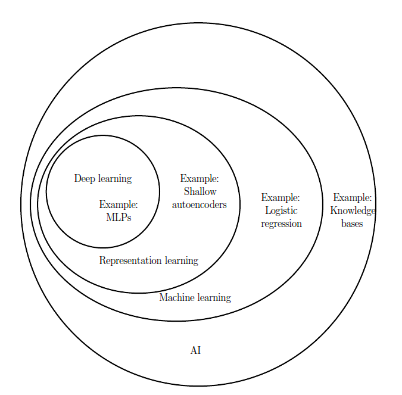
\includegraphics[width=0.6\textwidth]{figures/aprendizaje}
		\caption{Diagrama de Venn que muestra el marco de la \acrshort{ia}. Figura obtenida de~\cite{Goodfellow-et-al-2016}}
		\label{fig.aprendizaje}
	\end{center}
\end{figure}

En términos generales, la \acrshort{ia} contiene el Aprendizaje Máquina (\textit{Machine Learning}) definido como la capacidad de las computadoras para adquirir sus propios conocimientos, extrayendo patrones de datos sin procesar. A su vez, en el interior de la misma se sitúa el Aprendizaje de la Representación (\textit{Representation Learning}), que utiliza el aprendizaje máquina para descubrir, no sólo el mapeo de la representación a la salida, sino también la representación misma. Finalmente, en este último bloque sería situado el Aprendizaje Profundo (\textit{Deep~Learning}), que permite a la computadora construir conceptos complejos a partir de conceptos más sencillos.\\

Los algoritmos de aprendizaje profundo contrastan con otros en el número de transformaciones aplicadas a la señal mientras se propaga desde la capa de entrada a la capa de salida. Cada una de estas transformaciones incluye parámetros que se pueden entrenar como pesos y umbrales. A pesar de no existir un número fijo para este número de transformaciones, la mayoría de investigadores en el campo considera que este aprendizaje implica más de dos transformaciones intermedias~\cite{2014arXiv1404.7828S}. Además otro factor clave en este campo es el tamaño de las bases de datos utilizadas en el entrenamiento, teniendo que poseer una gran dimensión que permita realizar las funciones claves del mismo: análisis y síntesis.\\

Dentro del aprendizaje profundo, es posible aplicar diversas técnicas. La técnica más común y la que será empleada en este trabajo son las \acrfull{cnn}, que pretenden simular el funcionamiento del cerebro humano para establecer conclusiones sobre los datos introducidos a la misma. La idea básica es construir propiedades de que permitan crear modelos de redes invariantes a ciertas transformaciones en las entradas. Este tipo de redes tiene una estructura especial, mostrada en la Figura~\ref{fig.cnn}. La estructura indicada se compone, generalmente, por una capa convolucional, que implementa una operación de convolución, y una capa de submuestreo o agrrupación, que genera características invariantes de traducción calculando estadísticas de las activaciones de convolución a partir de un pequeño campo receptivo. Cada neurona en una capa oculta se conectará a un pequeño campo de la capa anterior, denominado campo receptivo local. En la capa convolucional, las neuronas están organizadas en múltiples capas ocultas paralelas, denominadas mapas de características, de tal manera que cada neurona en un mapa de características está conectada a un campo receptivo local. Para cada mapa de características, todas las neuronas comparten el mismo parámetro de peso que se conoce como filtro o \textit{kernel}~\cite{cnn}.

\begin{figure}[H]
	\begin{center}
		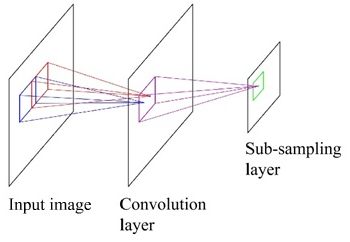
\includegraphics[width=0.4\textwidth]{figures/cnn}
		\caption{Estructura de \acrshort{cnn}. Figura obtenida de~\cite{cnn}}
		\label{fig.cnn}
	\end{center}
\end{figure}

El uso de este tipo de redes es muy variado, así como el tipo de entrada que se le puede introducir a la misma. En este caso, se centrará en la clasificación y detección de imágenes estáticas o en movimiento. La diferencia entre ambas aplicaciones es clara. La detección permite identificar en una única imagen diferentes objetos según el entrenamiento que se le haya proporcionado a la misma, mientras que la clasificación identifica una imagen entrante a la red como perteneciente a una clase determinada. Por otro lado, a pesar de que la aplicación desarrollada para la clasificación permite identificar una serie de dígitos en tiempo real, tanto el entrenamiento como la propia clasificación se realiza sobre imágenes estáticas, pues se introducen los diferentes \textit{frames} en la red. En el caso de la detección únicamente se trabaja con imágenes estáticas, pues el trabajo con imágenes en movimiento resulta demasiado complicado para la finalidad de este proyecto.\\

Por último, para implementar todo lo explicado anteriormente, existen múltiples plataformas que facilitan el entrenamiento y la implementación de estas redes. TensorFlow, Keras, Theano, Caffe, Lassagne o Torch son algunos de los ejemplos más conocidos de estas plataformas. En este trabajo se utilizará la plataforma Caffe, una de las más veteranas. La elección de esta plataforma radica en el gran número de ejemplos que proporciona la misma para poder implementar en las aplicaciones sin necesidad de realizar el entrenamiento, ahorrando tiempo al desarrollador. Además está centrado en la visión artificial, lugar hacia el que se enfoca este trabajo, y resulta bastante robusto y rápido.\\

Una vez se ha situado el trabajo en un marco definido, la motivación del mismo es clara. Se pretende ahondar en el mundo de la \acrshort{ia}, en concreto en técnicas de aprendizaje profundo y \acrshort{cnn}, para obtener resultados que puedan resultar interesantes y conseguir desarrollar una aplicación que permita implementar estas técnicas con la mayor exactitud posible. El interés por estas técnicas de aprendizaje profundo viene dado por su alto crecimiento actual y, sobre todo, por la gran ventaja que supone el no tener que extraer caracterísiticas de cada uno de los datos.

\section{Objetivos}
Los objetivos de este trabajo quedan claramente definidos y son los siguientes:
\begin{itemize}
	\item \textbf{Estudio y entendimiento de la plataforma Caffe.}. Se pretende entender la plataforma escogida para un correcto uso de la misma y la obtención de las redes que sean necesarias.
	\item \textbf{Entendimiento de la clasificación en Caffe.}
	\item \textbf{Desarrollo de componente que permita la clasificación de dígitos.}
	\item \textbf{Estudio y mejora de redes neuronales para la clasificación de dígitos.} Se realizarán diversas pruebas para tratar de alcanzar la red más robusta posible y poder utilizarla en el componente desarrollado.
	\item \textbf{Entendimiento y primera aproximación a la detección de Caffe.}
\end{itemize}

\section{Metodología}

Para el desarrollo de este trabajo, y la consecución de los objetivos, se ha seguido una clara metodología que ha dividido el trabajo en tres fases fundamentales. El primer paso fue definir claramente qué se quería conseguir con el mismo, qué mecanismos y técnicas se iban a utilizar y cuál sería la forma de trabajo. En esta primera fase se estableció el trabajo con la plataforma Caffe y el lenguaje de programación Python, ademas se marcaron los objetivos a alcanzar, mencionados anteriormente, y se definió una metodología de trabajo mediante reuniones semanales para poner en común las tareas realizadas y establecer algunas nuevas. Una vez superada esa fase, se procedió con el propio desarrollo del trabajo, avanzando de manera semanal sobre el mismo para alcanzar los objetivos marcados y analizar los resultados que fueron obtenidos. Esta fase tuvo la mayor importancia durante todo el desarrollo, pues, de manera simplificada, consiste en la propia elaboración del mismo. Como se indicó anteriormente, se establecieron reuniones semanales entre todos los miembros, estableciendo las pautas a seguir en el desarrollo y poniendo en común los resultados obtenidos. Una vez se fueron alcanzando los objetivos más importantes del proyecto se procedió con la fase de escritura de la memoria. Durante esta fase se volcarón los resultados obtenidos y se redactó de manera formal todo el proceso realizado. Esta fase no es excluyente, pues durante la redacción de la memoria se continuó avanzando con el desarrollo del trabajo, cumpliendo el resto de objetivos.\\

En la Figura~\ref{fig.diagrama} se desglosa, por semanas, el tiempo que ha llevado cada una de las fases, especificando el tiempo invertido para la consecución de cada uno de los objetivos.

\begin{figure}[H]
	\begin{center}
		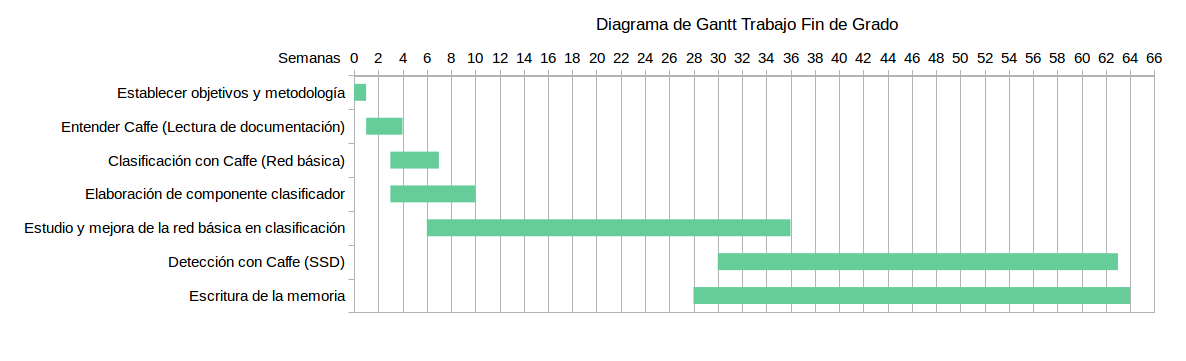
\includegraphics[width=1\textwidth]{figures/diagrama}
		\caption{Diagrama de Gantt del trabajo realizado}
		\label{fig.diagrama}
	\end{center}
\end{figure}

\section{Estructura de la memoria}
Para mostrar el trabajo realizado y los objetivos conseguidos se ha estructurado la memoria de la siguiente forma.

\begin{description}
	\item[Capítulo 1: Introducción y objetivos] \hfill 
	\vspace{5pt}
	\\
	En este capítulo se sitúa el trabajo en el marco actual de la tecnología, la \acrshort{ia} y la sociedad en general, para después establecer las metas que se pretenden alcanzar con el mismo. 
	\vspace{10pt}
	\item[Capítulo 2: Infraestructura] \hfill 
	\vspace{5pt}
	\\
	En este capítulo se procede a describir todo el \textit{Software} utilizado en el proyecto, incluyendo la principal plataforma, Caffe, y los conjuntos de datos empleados para la obtención y evaluación de las redes neuronales. Además se explican los diferentes parámetros que serán empleados para evaluar las prestaciones de las redes creadas.
	\vspace{10pt}
	\item[Capítulo 3: Clasificación con Aprendizaje Profundo ] \hfill 
	\vspace{5pt}
	\\
	Se expone todo el trabajo realizado para abordar el problema de la clasificación de dígitos con \acrshort{cnn}. En este capítulo se describe el funcionamiento de Caffe en esta tarea concreta, el componente creado, y todas las pruebas realizadas para tratar de conseguir una red robusta, con sus correspondientes resultados.
	\vspace{10pt}
	\item[Capítulo 4: Detección con Aprendizaje Profundo ] \hfill 
	\vspace{5pt}
	\\
	En este punto se proporciona la información necesaria para el entendimiento de la detección con la plataforma Caffe y se muestran algunos resultados de pequeñas pruebas realizadas para una mejor comprensión de la misma.
	\vspace{10pt}
	\item[Capítulo 5: Conclusiones y líneas futuras] \hfill 
	\vspace{5pt}
	\\
	Por último, se resumen todas las conclusiones obtenidas en los puntos anteriores y se establece un posible plan de actuación en un futuro para continuar la con la investigación en el tema que se aborda en el trabajo.
\end{description}